\section{Introduction}
During the last few month and years and since the revelation of Edward Snowden about the heavy use of secret service surveillance on users, privacy and security is a major concern in web applications. There is barley a week without discussion about saving private data of surveillance of phones or meta data. It is a time of discussions and fight over what is right, what should be possible, and what should be legal. Besides this the reality is "what can be done, will be done!". It were software developers who build the software for surveillance. The major Internet company's have a monopoly an meta- and user data and they use it for sell those date in a few microseconds to third party of services. The result is that users start to mistrust their devices and applications. This paper researches today's methods, concepts and technologies to secure user privacy. It describes what technologies are already here and what should be changed or improved to promote user privacy.

\newpage

\section{State Of The Art - Privacy}
\label{section:Introduction}
To describe methods for promoting privacy in web applications it is necessary to define privacy in technical terms. What techniques define and produce privacy and safety for users, and how did these techniques reach that goal.

\subsection{Concepts And Definitions Of Privacy and Security in Web Applications}

The concept of privacy and security has changed due to the fast rise of new technologies. Most of new technologies needs personal data from the user. Be it GPS coordinates to navigate to specific user related points or having access to calendars, emails and chat. Javaid describe security and privacy breaches as the "principles of exploiting vulnerabilities and finding system loopholes, control or access to a system" of “A measure of the exploitability of a weakness (\cite{javaid2013cyber}). Kabay writes about "A point where a system is susceptible to attack (\cite{kabay1996enterprise}) and to Blyth it is "Some weakness of a system that could allow security to be violated" (\cite{blyth2001information}). To provide more detail, the field of privacy and security can be divides into different subareas. The human side describes data theft, terrorism, omission (the share of secure data like passwords and access data) and the user abuse and fraud. The nature and environmental side lists physical and environmental conditions such as electromagnetic interferences or power fluctuations (\cite{javaid2013cyber}). The field that is most interesting for this research is the technical side. Here the list shows corruption by system errors or failures, data contamination, hardware failure, the insertion of malicious code and software or database modifications, installation errors and intrusion or unauthorized access, jamming and misrepresentation of identity and different types of system and application errors. This chapter concentrates highly on the technical side, with the knowledge in mind that many of the subareas are corresponding and depending on each other. Every part can be divided into three other chapters (\cite{rubinstein2012regulating}).

\begin{figure}[h!]
  \centering
      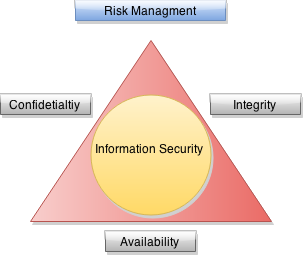
\includegraphics[width=0.4\textwidth]{images/figure1_0.png}
  \caption{Thread Triangle}
\end{figure}


The first area is confidentiality. Confidentiality in technical terms means the confidentiality in the application and the security and accuracy with which the application is produced. The app should be trustworthy of preventing eavesdropping, unnoticed notifications or intrusion and misrepresentation of identity. A short example is the authorized session in web applications with database support. It should not be possible to hijack a user session to get unauthorized access to private data. The session and the app should be aware of the identity of the user.

Integrity means a certain standard in which the user can trust. Systems with integrity act in a way that there behavior is predictable and of not surprising for users. System integrity is a vital point for confidentiality in a system from a users perspective.

Availability describes if a user can rely on an application and their behavior. Features for protection should be available at any time and not only in a certain technical states (\cite{zwingelberg2012privacy}).

"The triad of confidentiality, integrity, and availability has been widely accepted. While several extensions and refinements have been proposed, these core protection goals remained stable over decades and served as basis for many ICT security methodologies" (\cite{danezis2015privacy}).

\subsection{Privacy Enhanced Technologies In Web Applications}

\subsubsection{Privacy By Default}
"Development and integration of PETs means built-in privacy and the consideration of the full lifecycle of a system" \cite{danezis2015privacy}. Privacy Enhanced Technologies contains a large field of techniques. Build-in privacy means to protect personally identifiable informations (PII). Besides the argument for a global privacy standards to assist policy makers and developers, privacy by design is a key feature in the field of PET. The privacy by design approach was build upon 7 key principles and got adopted “as a holistic concept that may be applied to operations throughout an organization, end-to-end, including its information technology, business practices, processes, physical design and networked infrastructure" (\cite{danezis2015privacy}), by he International Conference of Data Protection and Privacy Commissioners.


\subparagraph{Proactive not reactive, Preventive, not Remedial} 
PbD should act proactive to prevent privacy issues. This means that it "prevents privacy invasive events before they happen. PbD does not wait for privacy risks to materialize, nor does it offer remedies for resolving privacy infractions once they have occurred. It aims to prevent them from occurring. In short, Privacy by Design comes before-the-fact, not after." (\cite{cavoukian2009privacy}). To achieve this, the application should aim for the highest level of protection possible. It should not rely on laws and regulations. It should aim to reach the highest possible protection. This also means a culture of continuous improvement and enhancement. It also means to recognize poor design standards and to correct them, even if the state of the art law did not require it at the point being.

\subparagraph{Privacy as the default}
An application should be maximal protective by default. This prevents user that did not have the technical interest or background, from exploiting their private security to others. In terms of confidentiality a user should be "certain of one thing, the default rule!" (\cite{cavoukian2009privacy}). If personal information is collected and used, the user should be aware of what is going on at all times. Also an application should be limited to the data that it needs for a special purpose. 

\subparagraph{Privacy Embedded into Design}
The design and architecture should be centered for user safety and privacy from the beginning. To achieve an embedding of this scale, there had to be standards and frameworks that support developers in this task. "Wherever possible, detailed privacy impact and risk assessments should be carried out and published, clearly documenting the privacy risks and all measures taken to mitigate those risks, including consideration of alternatives and the selection of metrics" (\cite{langheinrich2001privacy}).

\subparagraph{Full functionality, Positive Sum not Zero Sum}
Full functionality means to establish a win-win situation for all established interests and objectives. The opposite of this approach is a zero sum manner in which privacy has to compete against multiple other requirements such as security. The positive sum approach rejects these thesis and embraces to accommodate both into a functional design. "Privacy by Design avoids the pretense of false dichotomies, such as privacy vs. security, demonstrating that it is possible, and far more desirable, to have both.
" (\cite{cavoukian2009privacy}).

\subparagraph{End-to-end security, Lifecycle Protection}
User privacy has to be maintained and secured over the whole life cycle of the product. It should be handled like quality of reliability of a software product. In order to maintain this, an application needs to be responsible for personal information at every time and standards should assure the users privacy data.

\subparagraph{Visibility and Transparency}
Privacy by Design should be used on a fair information practice (FIP) basis. The user should be aware of what the application does at all times. For users it should be visible how and why an application use their data and what the application is doing with the data. Accountability for the user data, openness about policies and practices and compliance for procedures are the keywords. 

\subparagraph{Respect for User Privacy}
If an application is build around privacy interests the result for PbD is best. "Empowering data subjects to play an active role in the management of their own data may be the single most effective check against abuses and misuses of privacy and personal data" (\cite{cavoukian2009privacy}). The users free consent, the accuracy of personal information handling and total access to their own data is vital to include users in their own privacy.


\subsubsection{Privat Protection Goals} 
\footcite{hansen2012top} 
\footcite{rost2009datenschutz}
\footcite{probst2012generische}

Another enhancement strategy for protection privacy is to set goals. The \textit{Private Protection Goals} where proposed in 1999 and build a complement to the security triad in figure 1. The three basic goals where "embedded into a standardized data protection protocol acknowledged by the Data Protection Authorities in Germany, which proposed a usage on an European level (\cite{danezis2015privacy}). Besides the principle of \textit{unlinkability} there is \textit{transparency} and \textit{intervenability}. 

\subparagraph{Unlinkability}
Unlinkability means that privacy relevant user data should not be linked to other services or privacy related data. It means that different services should use different context to secure user data. A good example of a violation of this goals is the usage of cookies to identify users and track them to other services. Through those actions someone can learn about user behavior or common usage of websites, -services and habits. The given example make the issue of linkability more transparent.

A users visit a website or web service. To identify the user more easily and to make it more comfortable for the user to come back without loosing information, the side uses a cookie for the user e.g. if the user buy something and closes the website, the cart or buying list recognizes the user if he or she comes back by the cookie. This is a normal behavior and there is nothing bad about the use of cookies in such a way. A problem occur if the user visit another side and a third network or service can identify the user because of the cookie he gets from the last side. This assumes that the service or network has send a cookie from another side and recognize this cookie now on the new site. By this data linking, networks can learn meta data about users. Where does the user comes from? How often did a user visit a specific web service? Did the user use specific sites regularly? All information can be damaging the users privacy. It leads to connection point which can be used by e.g. ad networks to specified ads because of the knowledge where a user comes from or will go to. In data unlinkability such proceedings should not be possible. The user is safe because there will be no connection between different private data points.

Unlinkability is bind to the us of data minimization. Only data the application needs should be asked for. Through this the unwanted use, or use by mistake or coincidence of user related data can be avoided.


\subparagraph{Transparency}
The user should be aware of all things the application or service does with his or her data. In order to provide real transparency of the process the user should not only know what happens to the data at any time, the goal is that the user can understand how the data will be processed and for what purpose. To achieve this, the application or software has to be tailored for the special needs of the user that uses the program. It is necessary to use the users language and state of knowledge. It matters if your application is produced for a data controller or for a technically inexperienced user. Another part of this policy is proper documentation and the provision of the source code and a proper private policy. It should be understandable and maintainable to provide maximal openness to the process. The main focus of the transparency goal is the communication with the person whose data are processed. As explanation of this goal take a map applications which asks the user to store the GPS data. The software needs to be fully cooperative and open to the user. Why is the GPS location needed? Is it for navigational purposes or are there other processes going on in the application? What happen with the GPS data? Is it used locally or on a server? How long does the GPS location gets stored? The user has a right to know and the application needs to give the information freely so that the user needs not to search for an explanation, the explanation should be granted directly by the application. 

\subparagraph{Intervenability}
To complete the previous points, an application needs the possibility of intervention. If users can be sure about their unlinked private data and if they understand what is going on, they should intervene at any point during the process. This means: before, during and after the data procession and usage through the application. If a user have a change of mind, it should to be possible to revert steps or to set the software back to an earlier state and to delete already processed data. The users right to withdraw consent is a major point. At no time should a user be overturned by automated decisions, except the privacy by default logic. A good example about the goal of Intervenability is the users grand of request from an application to post to a social network. If the user grands the request, her or she should be allowed to stop it before, during and after data procession. If a user withdraw consent, all the data should be erased from the application and network. 


\subsubsection{The Platform for Privacy Preferences (P3P)}

In the last subsection this research covered the ground of what privacy and security means and what concepts, goals and methods are in place to achieve a maximum privacy and security for users. However these are constructs that have to be used to take an effect on user privacy. Web developers have to use this methods and ideas to protect users. It would be an advantage if system are in place that helps developers to do so. "What would be helpful is some kind of announcement system ..." (\cite{langheinrich2001privacy}). An announcement system that checks if the privacy settings of a user fits the privacy policy of a website or application. An appropriate comparison of the described technique is the use of robot.txt files on world wide web servers. The robot.txt provides the rules and a web robot can access these rules to traverse deeper into the side. A system like this is the Platform for Privacy Preferences project (P3P), developed in 2002 by the World Wide Web Consortium (W3C). This system with its latest version \textit{The Platform for Privacy Preferences 1.1} (P3P1.1) "... enables websites to express their privacy practices in a standard format that can be retrieved automatically and interpreted easily and by user agents" (\cite{cranor2002platform}). The P3P provides this information in machine readable XML format (P3P policy) with the following specifications:

\begin{itemize}
  \item A standard schema for data a website wish to collect
  \item A standard set of uses, recipients, data categories, and other privacy disclosures
  \item An XML format for expressing a privacy policy
  \item A means of associating privacy policies with web pages or sites and cookies
  \item A mechanism for transport in P3P policies over HTTP
\end{itemize} \cite{cranorplatform}

To be more precise the following example provides a better look at the P3P

\subparagraph{P3P Example Of Usage}

As an introduction to P3P, let us consider one common scenario that makes use of P3P. Claudia has decided to check out a store called CatalogExample, located at HTTP://www.catalog.example.com/. Let us assume that CatalogExample has placed P3P policies on all their pages, and that Claudia is using a Web browser with P3P built in.

Claudia types the address for CatalogExample into her Web browser. Her browser is able to automatically fetch the P3P policy for that page. The policy states that the only data the site collects on its home page is the data found in standard HTTP access logs. Now Claudia's Web browser checks this policy against the preferences Claudia has given it. Is this policy acceptable to her, or should she be notified? Let's assume that Claudia has told her browser that this is acceptable. In this case, the homepage is displayed normally, with no pop-up messages appearing. Perhaps her browser displays a small icon somewhere along the edge of its window to tell her that a privacy policy was given by the site, and that it matched her preferences.

Next, Claudia clicks on a link to the site's online catalog. The catalog section of the site has some more complex software behind it. This software uses cookies to implement a "shopping cart" feature. Since more information is being gathered in this section of the Web site, the Web server provides a separate P3P policy to cover this section of the site. Again, let's assume that this policy matches Claudia's preferences, so she gets no pop-up messages. Claudia continues and selects a few items she wishes to purchase. Then she proceeds to the checkout page.

The checkout page of CatalogExample requires some additional information: Claudia's name, address, credit card number, and telephone number. Another P3P policy is available that describes the data that is collected here and states that her data will be used only for completing the current transaction, her order.

Claudia's browser examines this P3P policy. Imagine that Claudia has told her browser that she wants to be warned whenever a site asks for her telephone number. In this case, the browser will pop up a message saying that this Web site is asking for her telephone number, and explaining the contents of the P3P statement. Claudia can then decide if this is acceptable to her. If it is acceptable, she can continue with her order; otherwise she can cancel the transaction.

Alternatively, Claudia could have told her browser that she wanted to be warned only if a site is asking for her telephone number and was going to give it to third parties and/or use it for uses other than completing the current transaction. In that case, she would have received no prompts from her browser at all, and she could proceed with completing her order. (\cite{wenning2006platform})


\section{Todays Techniques For User Safety And Privacy In Webdevelopment}
\label{section:Introduction}
This section researches state-of-the art standards of techniques in webdevelopment to promote user safety in backend- and frontend development (\cite{Keerthi2014})

\subsection{Software Patterns And Technologies For User Safety And Privacy}
Finding and using proper methods and technologies for safety and privacy enhancement can be a challenge for developers and software architects. There is a constant potential of conflicts and inconsistencies between system requirements, privacy objectives and complexity of technology. To combine all these specifications it is advised to use established or proven software architecture and patterns. By using proven designs the developed software is less error prone (\cite{danezis2015privacy}). Architecture and software patterns reducing the complexity of the task and establish abstraction by eliminating unnecessary details that does not matter for the task at hand (\cite{antignac2014privacy}).

Independent from the choice of programming language there are key criteria that had to be taken into context.

\subparagraph{Trust assumption} Trust is a relationship between different parties about personal data. From a technical point trust without verification is a weak solution, because there is no possibility of prove if a party behaves after the determined rules. Other options of trust are that trust is granted by default but verifications can be carried out by any party, to check for violations. The opposite method is a no trust option in which cryptographic algorithms or protocols monitor the desired property (\cite{antignac2014privacy}). Known methods for are:

\begin{itemize}
  \item Zero knowledge proof (\cite{goldreichdefinitions})  
  \item Secure multiparty computation (\cite{lindell2009secure})
  \item Homomorphic encryption (\cite{gentry2009fully})
\end{itemize}

The \textit{ZKP} and \textit{SMC} are working similar. They try to evaluate a mathematical true statement without using private information of one of the two parties. Basically the method works by knowing and identify that, what the other party states, is true or false. \textit{Homomorphic encryption} uses ciphertext to encrypt for example a message. Both party's can decrypt the ciphertext with a public key.

\subparagraph{User Involvement} describes in what form, how and when an interaction with the user should take place. What can the user contribute to the system to make it better. If users are involved it is vital that they are aware an able to fulfill there rights as a user, like corrections, deletion and post denial of access.

\subparagraph{Technical Constraints} are system-, environmental-, user or software bind and describe limitations by some or all of the party's to fulfill a given task. If for example data has to be stored to a certain area or system there will be limitation to access or update this data.

\subsubsection{Design Strategies And Software Patterns}
There are different software patterns for different tasks. Patterns are useful to "provide a scheme for refining the subsystems of components of a software system, of the relationship between them. It describes a commonly recurring structure of communication components that solve a general design problem within a particular context" (\cite{buschmann1996pattern}). Since our context is privacy and safety we have to provide patterns for this specific task. The following explanation and list of patterns for privacy are not complete. There are only a few Patterns that are specialized for privacy enhancement, but other patterns fulfill these task too, even if they are not described as PE Patterns. In case of this research different software Patterns are combined with Design strategies to make sense in the privacy context.

\subparagraph{Data Oriented Strategies}

\subparagraph{MINIMISE Design Strategy}
The MINIMISE strategy focuses on limiting the amount of personal data that is stored, collected or included (\cite{domingo1997multi}). This means no unnecessary data should be collected and a service or application has to reason why data is collected and for which purpose (\cite{graf2010pattern}). Established software pattern for the MINIMISE design are \textit{select before you collect} (\cite{jacobs2005select}) or \textit{anonymisation and use pseudonyms} (\cite{pfitzmann2008anonymity})


\subparagraph{HIDE Design Strategy}
HIDE functioned by hiding all plain information for anybody. It is not specific about from whom to hide, because often plain information develop during the use of an application (the best example is the hidden password. The user itself cannot see the password). If plain information develop during the use of a service they can be used as identifiers. Famous examples are RFID Tags or a IP address. They are not hidden and are in danger to get abused for unwanted operations (\cite{domingo1997multi}). Patterns for this strategy are all sorts of encrypting data during storage or transfer (\cite{chaum1981untraceable})


\subparagraph{SEPARATE Design Strategy}
By decentralize data in applications and webservices it is harder to link specific sets of data to a person. The SEPARATE strategy states that data should be stored locally whenever possible. Services like Facebook or Google+ are working centralized. It it the opposite of a privacy friendly approach and therefore the SEPARATE strategy often gets forgotten or not used (\cite{danezis2015privacy}).
This could be the reason that there are no actual linked or use patterns for this design strategy. 

\subparagraph{AGGREGATE Design Strategy}
Aggregation of data means to aim for the sum of the data, not details of the data. This will restrict the amount of personal data on the one hand, but comes with less sensitivity about the data. Known patterns for the AGGREGATE strategy are \textit{aggregation over time }, \textit{dynamic location granularity}, \textit{k-anonymity} (\cite{sweeney2002k}) and \textit{differential privacy} (\cite{fahl2013rethinking})


\subparagraph{Process Oriented Strategy}

\subparagraph{INFORM Design Strategy}
The main goal of the INFORM strategy is to provide transparency and openness to to the user of a system. The user of a service should be informed how the system security works and which third parties are informed about the date he or she share with the application. INFORM strategy also makes sure that. The introduced \textit{privacy preference} of the W3C could serve as a pattern example for the INFORM strategy (\cite{graf2010pattern}). 

\subparagraph{CONTROL Design Strategy}
This strategy implements control over personal data and builds an important counterpart to the INFORM strategy. If a user is proper informed about what personal data is processed he or she can choose what permit or deny services and request. Without INFORM the CONTROL is limited.\textit{end-to-end encryption} is a fitting software pattern for the CONTROL strategy  

\subparagraph{ENFORCE Design Strategy}
The statement of the ENFORCE strategy is that it should be a privacy policy in place. A privacy policy informs the user about important steps about the application and shows that technical protection against violations is in place for the user. A typical pattern for ENFORCE is \textit{access control}, \textit{privacy rights management} and \textit{sticky policies}.

\subparagraph{DEMONSTRATE Design Strategy}
Is an extension of the ENFORCE strategy. It requires that a data controller proves that it is in control of the data. For this a privacy policy like in the ENFORCE strategy is necessary. DEMONSTRATE has to show how this policy is implemented and in case of breaches how it behaves (\cite{langheinrich2001privacy}). Logging and auditing are examples for DEMONSTRATE patterns (\cite{katsikas2005trust}).

\section{Privacy Techniques}
 
 This section describes in Detail which privacy techniques are available and mature for todays developers. It begins with authentication of user actions and explains the possibilities of secure communication and basic techniques of encryption and pseudonymisation. The last part of this section describes privacy in databases.

 \subsection{Authentication And Secure Communications}

 The key element of a secure and private communication between users and services is a state of the art authentication. Authentication is the process of identifying one self to a system or another user, to get privileged access to information and actions that are restricted. Since authentication is often the starting point for interactions with applications and services, a strong and reliable authentication is necessary to prevent privacy threats through tracking or hijacking a users identity (\cite{danezis2015privacy}). A state-of-the art authentication should be enable protection against the passive observation of the identity of a user or what the user is doing (tracking user actions). Another risk is that a confused user can be persuated to authenticate to the wrong service and therefore leak private informations. The attempt to convince a user to leak private data and identity is know as "pishing attack" (\cite{dhamija2006phishing}).
 The goal of an authentication is to prevent third party's of any kind from interfering into sessions or communications between users or services and keep a link between them secure, so that both sides can establish trust and share information and actions.

 % figure how a pishing attack works

 To establish such a link between both sides it is state of the art to use \textit{end-to-end} communication since it comes with many benefits. A useful technique for end-to-end authentication is \textit{Just Fast Keying (JFK)} (\cite{aiello2004just}) which allows imitation and responder privacy in an end-to-end communication.

 % figure of end-to-end with responder and initiator 

\textit{JFK} consists of two variations. \textit{JFKi} provides privacy for the initiator of the communication. \textit{JFKr} is the counterpart and protects the responder of the end-to-end communication. If both \textit{JFK} are established the party can be trusted that they are talking to the one they expect. This happens through the use of certificates and public key cryptography derived with a new session from the \textit{JFK}. On Benefit of the \textit{JFK}is that it is simple to use but reaches its design goals.

\subsubsection{Design Goals of Just Fast Keying}

\begin{itemize}
  \item Security: No one other than the participants may have access to the generated key
  \item PFS: JFK provide Perfect Forward Security
  \item Privacy: It must preserver the privacy of the initiator and/or responder, as far as possible
  \item Memory-DoS: It must resist memory exhaustion attacks
  \item Computation-DoS: It must resist CPU exhaust attacks
  \item Availability: It must protect against observers that would like to interfere in transmitted packages
  \item Non-Negotiated: It mus avoid complex negotiations over capabilities
  \item Simplicity: It should be as simple as possible within constraints and requirements
\end{itemize} \cite{canetti2002universally}

\textit{PFS - Perfect Forward Security} requires a long term key which is not effected if compromised in there security. According to Aiello and Bellovin, \textit{PFS} is arguable. Nevertheless \textit{JFK} protects against third party's no matter if the planed connection is successful or unsuccessful. A third party can not identify who an initiator or responder is. \textit{Just Fast Keying} fulfills the requirements of authenticity, integrity and confidentiality and provides state-of-the-art privacy. 

To reach these goals \textit{JFK} uses different techniques. First both party's exchange a \textit{Shared Secret} that is only known by the two participants.

\begin{figure}[h!]
  \centering
      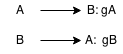
\includegraphics[width=0.2\textwidth]{images/sharedsecret.png}
  \caption{Shared Secret between A and B}
\end{figure}

The \textit{Shared Secret} is based on the \textit{Diffie Hellman Key Exchange} which exchanges a secure cryptographic key over public channels. The \textit{DH} can be explained with the famous Alice and Bob example. Alice and Bob have colors. Both have a common white color, and a secret color which is only know by themselves. Alice and Bob want to share the secret color. To do this they publicly share the common white color mixed with their secret color. Because they both know that they have the color white as the common color, they can extract the secret color of the other party. A third party don't know what the common color is and therefore a separation of the colors by trial and error would be very expensive. Now Alice and Bob have both the secret color of the opposite side. The have a common secret (\cite{al2000diffie}).

After sharing a common secret the \textit{JFK} forces a challenge response which means that A gets an element back that is signed by the private key of B and vice versa. Now both party's know that the opposite side is the person or group that they claim. The \textit{JFKr} now uses encryption to ensure identity protection. The last part is the use of a DoS protection to secure the connection.

A weaker form of this authentication is the use of a username-password system. This technique is common in web services. In this case the authentication presumes that through the knowledge of a username and a secret password, the user is the person he or she claims to be. However \textit{pishing attacks} or unexperienced and confused users can be in danger. Username-Password systems should be used with great care. Encryption of the communication data is necessary and web services should use \textit{TLS} protocols or \textit{HTTPS Forms} to encrypt the communication \cite{bonneau2012quest}. Most of the web services are based on \textit{Client-Server} structure whereas end-to-end authentication allows direct verification of party's, users or groups.  

\subsection{Single Sign On And Federated Systems}
Federated management systems providing a \textit{Single Sign On} service that make it possible to enroll users to other services by identifying them or telling other services that the user is the one he claims. \textit{SSO} services identify users for other services. This methodology supports the minimalism principle that this paper explains earlier. As an example take a online library which needs to identify students who borrow books. To do this in a minimalistic approach the library do not need to know exact user data. It is sufficient to only know the university membership status to decide if a student is allowed to borrow books. For good privacy protection data minimalism is a vital point. Context data like an id or the age and address produce meta data, which can be tracked and linked to learn about users. Implementing \textit{Federated Management Systems} prevent meta data and support user privacy (\cite{alsaleh2006enhancing}). A good real world application that uses a \textit{Federated Identity Management} is Facebook, Google plus, Twitter and other social networks. Today there are many services and applications where a user can login with an existing social media account. The service did not require other data than the membership of this specific social network. In this use case facebook or one of the other networks now the user and share only that it is a real person. If a user is a valid member of such a network he or she had to agree on their policy. A service which allows \textit{Single Sign On} through a social network can be sure that this specific user agreed to this policy and therefore knows enough about the user to accept him or her. Even if the application did not know any other meta data. 

% figure of federated systems
% \begin{figure}[h!]
%   \centering
%       \includegraphics[width=0.5\textwidth]{images/??}
%   \caption{Shared Secret between A and B}
% \end{figure}

\subsection{Attribute Based Credentials}
The downside of the above described \textit{SSO} is that, in this case, the social network knows anything or at least very much about their users. The \textit{Identity Provider - IdP} of the network becomes a "spider in the web for all identity-related transactions" (\cite{danezis2015privacy}). This, in fact is the opposite of the stated user privacy a web service should provide, because it leads to several security, privacy and usability concerns (\cite{alpar2011identity}). To achieve both, user protection and a \textit{SSO} via \textit{IdP}, \textit{Attribute Based Credentials - ABC} are the solution. The principles of \textit{ABC} are basically the same than with a normal \textit{IdP} but there is protection from changing the scope and use different \textit{IdP} to produce as little meta data as possible. Attributes of a user, like hair color, name, age, gender, grades, subscriptions and many others are identified by sources that are predestined to know this attributes and are trustworthy. A Highschool, for example,
 is a reliable source for diplomas and grades, a hospital or the government are reliable about the date of birth. By spreading the scope over different sources, which did not know the attributes other sources know, a huge amount of meta data can be prevented. To be a valid source for user attributes there have to be certain properties that needs to be fulfilled. 

\subparagraph{Unforgeability}
\label{subp:subparagraph_name}
Only a suitable service can produce a credential. A credential should not be forgeable by other sources, and should involve only attributes that are valid.

\subparagraph{Unlinkability}
\label{subp:unlinkability}
Only the prover of the credential can link the user to this credential. No other party or service should know about this link. Even if a user uses a credential hundreds of times to register, the service provider should not be aware that this specific user authenticate. A user should stay anonymous to a service provider.

\subparagraph{Non-transferability}
\label{subp:non_transerability}
The credential should only be usable by only one user. Identity share should not be possible. Also a user should not be allowed to combine credentials, to get access to groups he or she did not belong to.

\subparagraph{Revocability}
\label{subp:revocability}
A credential should be revocable. If a credential gets be revoked non of the verifiers should accept it anymore.

\subparagraph{Black listing}
\label{subp:black_listing}
A trusted inspector should have the power to blacklist misbehaving users an. In this case the unlinkability is in danger. (\cite{tsang2011nymble})

(\cite{chaum1985security})
(\cite{camenisch2001efficient})

Good examples are \textit{U-Prove} from \textit{Microsoft} and \textit{Idemix} from \textit{IBM}. \textit{U-Prove} uses a \textit{Blind Signature Protocol} (\cite{chaum1983blind}). While \textit{U-Prove} is efficient implementable, but needs the user to be online to obtain refreshed credentials \textit{Idemix} is the opposite. It is hard to implement, but the user did not need to be online. In contrast do Microsoft, IBM uses the \textit{Zero Knowledge Proof} for \textit{Idemix} (\cite{camenisch2001efficient}). Today no real efficient \textit{ABC} system exists. Hardware support and the use of self-blindable credentials could change this in the near future (\cite{batina2010developing}). 


\subsection{Secure Private Communication} 
\label{sub:secure_private_communication}
Secure communication is a major part in privacy since nearly everything on the word wide web has to do with communication in different forms. Be it voice over IP or data messenger systems like \textit{Facebook Messenger} or \textit{WhatsApp}. Communication ca be established between users or users and service. Because most of the physical networks today provide poor guarantees for privacy confidentiality every communication should be encrypted, even messages or data that is public and without security relevant content should be encrypted because of the power of meta data to link and connect single events and data to more detailed picture of a user (\cite{fawcett1996combining}).

\subparagraph{Client-Service Communication}
To deploy a confidential network for communication from a client to a service both party s needs to be truth each other (like mentioned above). To implement and configure such a network it is the best practice today to use security features like \textit{Transport Security Layer, TLS} (\cite{dierks2008transport}) or the \textit{SSH Secure Shell Protocol} (\cite{barrett2005ssh}) which are both good implementable and known as mature technologies. \textit{TLS} and \textit{SSH} belong to the family of \textit{Public Key Cryptography}. The downside of both services is that if on party is compromised, the whole channel is compromised and therefore not private anymore. Another difficulty is that \textit{SSH} relies on a manual verification, which some users might not be capable of. But even with this difficulty's, the deployment of \textit{TLS} (version 1.2) should be considered as state-of-the art in todays network communications.

\subparagraph{End-To-End Communication}
Services like messengers, social networks, voice over IP \textit{WoIP} or email are known as end-to-end communication. In this context end-to-end means that only two sides hold the trust and identification of where the other party is and if it is trustworthy. Knowing this, private data or keys should only be available for the end users on their devices. They should not hold at the service provider since this will damage the \textit{Unlinkability} principle mentioned earlier. In the field of end-to-end communication the standard technologies are \textit{The Pretty Good Privacy - PGP} (\cite{zimmermann1995official}) and the \textit{Secure/Multipurpose Internet Mail Extensions - S/MIME} standard \cite{ramsdell1999s}. Both methods are using \textit{Public Key Cryptography} like \textit{TLS} and \textit{SSH} and suffer the same downsides but like the client-service techniques are considered as todays standard.

\subparagraph{How Public Key Cryptography Works}
There are many other services and techniques to protect user privacy but the before mentioned four are todays state-of-the art techniques. They all use \textit{Public Key Crypthography} which this sub chapter will explain in basic with \textit{PGP}. 

\subsubsection{Encryption}
To encrypt data or a message you with \textit{Public Key Cryptography} the user has a private key and a pubic key. The public key can be shared and anyone with this public key (which is bind to the private key) can encrypt messages and date. In \textit{PGP} the plain text of a user message gets encrypted with a random created session key. This random key gets encrypted with the public key. Both systems produce the key by creating a \textit{Hash} file which has certain characteristics like length. The \textit{Hash} should not be altered, because otherwise a decryption is not possible. The produces \textit{Ciphertext} is now send to another person and is now encrypted. No third party can decrypt it without the private key.

\subsubsection{Decryption}
The encrypted message now has an encrypted session key (random key) and the ciphertext. To decrypt the message the recipient has to use the private key that fits the shared public key. With this the recipient can decrypt the session key. The session key is used to decrypt the ciphertext to the original plain text again. 

\begin{figure}[h!]
  \centering
      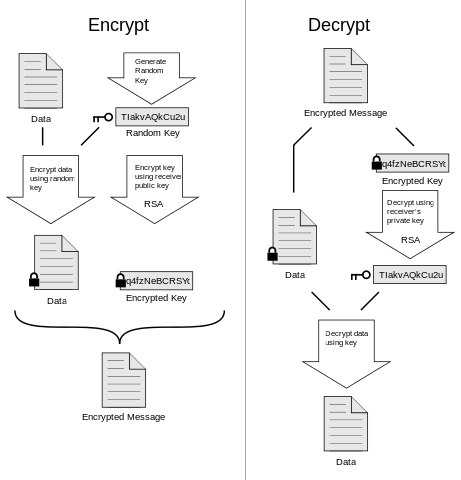
\includegraphics[width=0.5\textwidth]{images/pgp.png}
  \caption{PGP Encryption/Decryption} 
\end{figure}

Graphic by \url{http://en.wikipedia.org/wiki/Pretty_Good_Privacy#/media/File:PGP_diagram.svg}

  
\subsection{Anonymous Communication Family's} % (fold)
\label{sub:anonymous_communication_families}
In anonymous communication there are several family's. They all try to protect and secure communication but do this on different approaches and with different methods. Private communication needs two things to be sufficient and secure. First, no one can hide their own identity themselves in communications. The user needs software and services that does this for him or her. Second, "anonymity needs company" \cite{dingledine2006anonymity}. If a user uses a network to protect his or her privacy it best to use networks with many users. More users in a communication systems means a better anonymity. This cite can be best represented by the comparison between large city's ans small villages. In small villages nearly everyone knows anyone and therefore there is not much data needed to identify a specific person. This task gets more complicated in a huge city where the meta data can fit to different persons and therefore are no longer unique to identify a specific person.

\subparagraph{Onion Routing}
Onion Routing mean that communication data uses multiple relays and stations (\cite{goldschlag1999onion}). If a single route can be observed easily it is very hard to maintain the observation of many routes and stations which are also changing with every new communications session. The \textit{TOR} network is a good example for \textit{Onion Routing} (\cite{dingledine2004tor}). The \textit{TOR} network uses more than 5000 relay stations and servers over 1 million users per day. It fulfiller the need of a huge company which makes it harder for observers to detect a single user and provides many relays (\cite{danezis2015privacy}). Even if the \textit{TOR} network is well configured it is still possible to detect which user is talking to which through statistical analysis. 

\subparagraph{Proxies}
Single proxies are a simpler way to for anonymous communication but not as secure as \textit{Onion Routing}. It only uses one \textit{Proxy} which addresses the traffic of the communication so that other party's cannot immediately see where the source of the communication is situated. a an additional security layer encryption of the message should be considered.

\subparagraph{Mixed Networks}
\textit{Mixed Networks} trying to restrict the message size to a specific and uniform amount as addition to the use of multiple relays executed by the \textit{Onion Routing} (\cite{chaum1981untraceable}). This makes it much harder to identify a persons in the network through statistical analysis , because everyone has the same "size" of messages.

\subparagraph{Broadcast Schemes}
A expensive but simple technique is \textit{Broadcast Schemes}. With this method every messages gets send out to all members of the communications group. Every member has to decrypt the message to see if the messages is relevant to him or her (\cite{stajano2000cocaine}).

\subparagraph{Steganography}
The last presented family is the method of \textit{Steganography} which means to hide your identity by masquerade the services and routes you are using. It basically comes down to the attempt that online traffic looks like other traffic and is not interesting enough to third party's, that try do find relevant and user related data (\cite{katzenbeisser2000information}).

\subsubsection{Privacy In Databases}
\label{ssub:privacy_in_databases}
Another major subject is privacy in databases, since they are used widely and are essential to many web- and user related services. Privacy in databases can be understood as protecting where the owner of the database is and that records are not transferred to other services, like insurance company's or other third parties who look for meta data. For database privacy the subject can be split into three groups.

\subparagraph{Responder Privacy} is preventing identification or re-identification how database records are linked to each other. This produces meta data if, for example tables with names or age are linked to tables with diseases or other data that can produce assumptions about an individual.

\subparagraph{Owner Privacy} means that two individuals or services process data from the database, but only the result of the query gets revealed (\cite{danezis2015privacy})

\subparagraph{User Privacy} on the other hand, is the prevention of leaking query's and to protect against profiling and re-identification of a user.

Basically the protection of databases follows the same principles as in communication or other data. It should be consider data minimalistic and unlinkability leak as little as possible meta data that can be processed.

\section{Conclusion}
This research looked at different aspects of user privacy for web related services and application. Starting with the concepts of what privacy and security in web applications is and how it can be established, to the wide field of privacy enhancement with standardized privacy goals, this paper researched the technologies that can be used in todays development processes to make an application secure and more private for users. There are many good concepts like the \textit{Platform For Privacy Preferences P3P} or the \textit{Privacy By Default} thesis. Not all are mature enough to go into todays development processes of applications, like the \textit{Attribute Based Credentials}. However, there are concepts and techniques available, that should be used in a standard and widely approached way. The most of todays applications did not use the \textit{Privacy By Default} principle or the general goals for privacy protection. \textit{PGP} and \textit{SSH} are still used by either developers, or more educated users. This could mean that most of the average users did not use encryption methods for communication. The goal is to  make the use of those techniques easier or to implement them into applications, in a way that the enduser did not need to become an technical expert. One of the major problems is the shift of knowledge in technology. Technology evolves fast and there is danger that certain users are left behind, because they cannot update their knowledge of technology and they don't have the ability to do so. The gap of knowledge between tech savvy persons and end users is getting bigger. It is the responsibility of developers to use todays techniques to protect their users and to build software that is transparent for users. This means that in the future more of the described techniques should be used. The focus should on privacy by default could because this could help to prevent users from leaking private information. Right now there are several techniques ready and mature to be used, but they lack either the fastness or the simpleness a user needs to use them properly and on a daily basis.